\section{Аппаратура управления}

В этой главе мы подробно рассмотрим устройство и настройку аппаратуры радиоуправления FlySky FS-i6S, которая входит в стандартный комплект образовательного квадрокоптера «Геоскан Пионер». Пульт дистанционного управления (аппаратура) — это основной инструмент внешнего пилота, позволяющий контролировать полет, переключать режимы работы и выполнять настройку параметров дрона на расстоянии.

Аппаратура работает в паре с приемником, установленным на борту квадрокоптера, передавая команды по радиоканалу. Для корректной работы системы необходимо правильно настроить пульт и установить связь с приемником.

\subsection{Настройка пульта}

Перед первым использованием или после сброса настроек необходимо сконфигурировать пульт управления. Это обеспечит правильную интерпретацию команд полетным контроллером.

Для настройки пульта выполните следующие действия шаг за шагом:

\begin{enumerate}
    \item Вставьте батарейки (4 шт. типа AA) в батарейный отсек и включите пульт дистанционного управления. Для включения необходимо нажать одновременно две кнопки питания (расположены в центре лицевой панели) и удерживать их до включения экрана.
    \item После загрузки на дисплее появится главный экран с отображением текущего состояния, напряжения батарей и положения стиков.
\end{enumerate}

\begin{hintbox}
    \textbf{Подсказка:} В целях безопасности пульт проверяет положение переключателей при включении. Если на экране отображается предупреждение «Warning!!! Place all switches in their up position», это означает, что один из тумблеров находится в активном состоянии или стик газа не в нуле. Приведите все переключатели в верхнее положение (от себя), а левый стик (газ) опустите в самое нижнее положение.
\end{hintbox}

\begin{figure}[H]
    \centering
    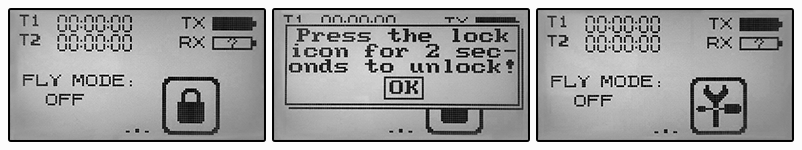
\includegraphics[width=0.8\textwidth]{images/rc_setting_main.png}
    \caption{Главный экран пульта управления FS-i6S}
\end{figure}

\begin{enumerate}
    \setcounter{enumi}{2}
    \item Изначально сенсорный экран заблокирован от случайных нажатий, о чём сигнализирует иконка замка в нижнем правом углу. Для разблокировки нажмите на иконку и удерживайте её в течении 2-4 секунд. После разблокировки иконка сменится на изображение гаечного ключа.
    \item Нажмите на иконку с гаечным ключом, чтобы попасть в меню настроек. Меню разделено на две основные вкладки:
    \begin{itemize}
        \item \textbf{FUNCTION} — здесь производится настройка функций самого пульта (каналы, реверсы и т.д.).
        \item \textbf{SYSTEM} — отвечает за системные настройки связи и приемника.
    \end{itemize}
\end{enumerate}

\subsubsection{Настройки вкладки FUNCTION}

В этой вкладке мы настроим назначение каналов и направление их работы. Это критически важно для того, чтобы движения стиков и переключения тумблеров вызывали ожидаемую реакцию дрона.

Для работы с «Пионером» выполните следующие настройки:

\begin{enumerate}
    \item \textbf{Настройка реверса каналов (Reverse):}
    \begin{itemize}
        \item Перейдите в меню \textbf{REVERSE}.
        \item Установите каналы \textbf{Ch2} (Тангаж) и \textbf{Ch4} (Рыскание) в положение \textbf{Rev} (Реверс). Остальные каналы оставьте в Norm.
    \end{itemize}
    
    \item \textbf{Настройка вспомогательных каналов (Aux. Channels):}
    Для управления режимами полета и дополнительными функциями необходимо назначить физические тумблеры на логические каналы пульта. Перейдите в меню \textbf{AUX. CHANNELS} и настройте каналы следующим образом:
    \begin{itemize}
        \item \textbf{Channel 5:} Нажмите на кнопку выбора канала. В окне \textbf{CH TYPE} выберите \textbf{SWx} (переключатель). Затем нажмите на надпись SwA (по умолчанию) и в открывшемся списке выберите тумблер \textbf{SwC} (трехпозиционный переключатель справа). Этот канал обычно используется для смены режимов полета.
        \item \textbf{Channel 6:} Аналогично настройте на тумблер \textbf{SwD} (крайний правый переключатель).
        \item \textbf{Channel 7:} Настройте на тумблер \textbf{SwB} (трехпозиционный переключатель слева).
        \item \textbf{Channel 8:} Настройте на тумблер \textbf{SwA} (крайний левый переключатель).
    \end{itemize}
\end{enumerate}

\begin{figure}[H]
    \centering
    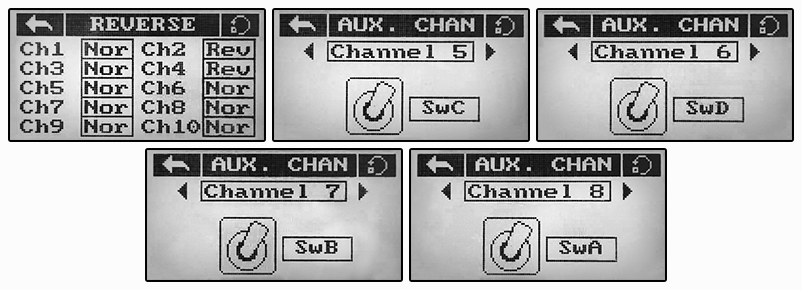
\includegraphics[width=0.8\textwidth]{images/rc_setting_aux.png}
    \caption{Меню настройки вспомогательных каналов}
\end{figure}

\subsubsection{Настройка вкладки SYSTEM}

В этой вкладке задаются параметры протокола передачи данных и режим работы стиков.

\begin{enumerate}
    \item \textbf{Выбор протокола выхода (Output Mode):}
    \begin{itemize}
        \item Перейдите в меню \textbf{OUTPUT MODE}.
        \item Убедитесь, что в поле \textbf{Output} выбран протокол \textbf{PPM}. Полетный контроллер «Пионера» настроен на прием сигналов именно в этом формате. Также должен быть выбран режим \textbf{S.BUS} в поле Serial, если используется соответствующее подключение, но для базовой настройки PPM является основным.
    \end{itemize}
    
    \item \textbf{Режим стиков (Sticks Mode):}
    \begin{itemize}
        \item Перейдите в меню \textbf{STICKS MODE}.
        \item Выберите режим \textbf{M2 (Mode 2)}. В этом режиме левый стик отвечает за Газ (вверх/вниз) и Рыскание (влево/вправо), а правый — за Тангаж (вперед/назад) и Крен (влево/вправо). Это наиболее распространенная схема управления для квадрокоптеров.
    \end{itemize}
\end{enumerate}

\begin{figure}[H]
    \centering
    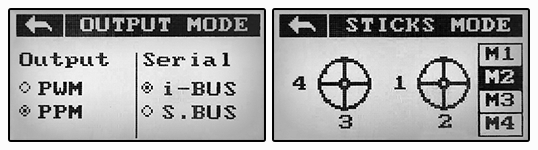
\includegraphics[width=0.8\textwidth]{images/rc_setting_system.png}
    \caption{Системные настройки: выбор режима PPM и Mode 2}
\end{figure}

\subsection{Связь пульта с приемником}

Процедура привязки (Binding) необходима для того, чтобы приемник, установленный на квадрокоптере, «узнал» ваш пульт и реагировал только на его команды. Это исключает пересечение сигналов при полетах нескольких дронов одновременно.

\begin{warnbox}
    \textbf{Внимание:} Для использования квадрокоптера «Пионер Мини» с пультом радиоуправления, в автопилот должны быть загружены соответствующие параметры! Без этого дрон может не реагировать на команды.
\end{warnbox}

\subsubsection{Процедура привязки}

Выполните следующие действия для сопряжения устройств:

\begin{enumerate}
    \item Убедитесь, что приемник (FS-A8S или аналогичный) подключен к плате автопилота.
    \item Найдите на корпусе приемника маленькую кнопку с подписью \textbf{«BIND»}. Нажмите её и \textbf{удерживайте}.
    \item \textbf{Не отпуская} кнопку BIND, подайте питание на квадрокоптер (подключите аккумулятор).
    \item После подачи питания светодиод на приемнике должен начать \textbf{быстро мигать}. Это означает, что приемник перешел в режим привязки. Теперь кнопку можно отпустить.
    \item Включите пульт управления. Зайдите в меню настроек (\textbf{SYSTEM}) и выберите пункт \textbf{RX Bind}.
    \item На экране пульта появится надпись \textbf{Binding to RX...}. В этот момент пульт ищет приемник в режиме привязки.
    \item Как только связь установится, светодиод на приемнике начнет \textbf{мигать медленно}.
    \item Для завершения процедуры нажмите иконку «Назад» ($\leftarrow$) на пульте, чтобы выйти из меню RX Bind.
    \item После выхода из режима привязки светодиод на приемнике должен загореться \textbf{постоянным светом} (красным). Это подтверждает успешное сопряжение и наличие стабильной связи.
\end{enumerate}

\begin{warnbox}
    \textbf{Важно:} Чтобы избежать конфликтов управления, связывайте только один пульт с одним приемником. Если вы меняете пульт или приемник, процедуру привязки необходимо повторить.
\end{warnbox}

\begin{figure}[H]
    \centering
    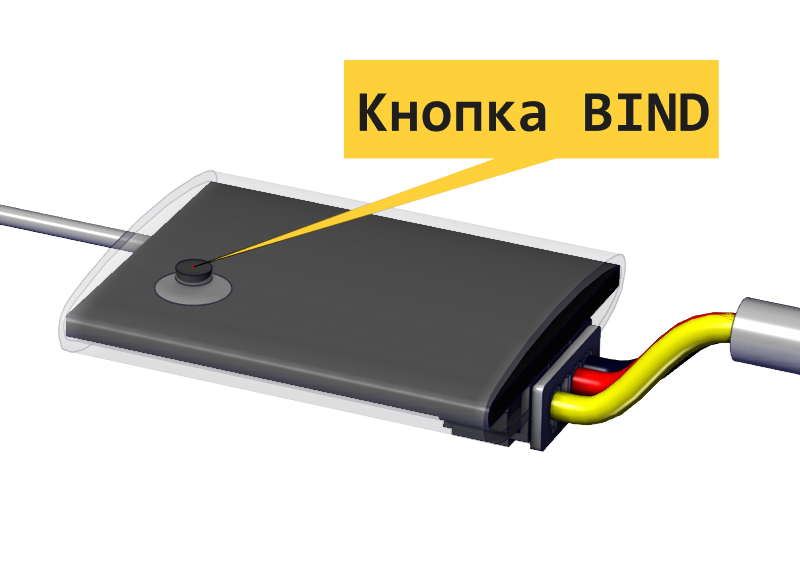
\includegraphics[width=0.6\textwidth]{images/FS-A8S_bind.png}
    \caption{Приемник FS-A8S: расположение кнопки BIND}
\end{figure}

\subsubsection{Возможные проблемы и их решение}

Если после выполнения процедуры квадрокоптер не реагирует на команды:

\begin{itemize}
    \item \textbf{Проверьте протокол:} Зайдите в настройки пульта \textbf{OUTPUT MODE} и убедитесь, что выбран \textbf{PPM}. Другие протоколы (например, PWM или i-BUS) могут не восприниматься текущей прошивкой автопилота без дополнительной настройки.
    \item \textbf{Повторите привязку:} Возможно, вы отпустили кнопку BIND слишком рано или не успели включить режим привязки на пульте. Попробуйте снова.
    \item \textbf{Проверьте параметры:} Если вы летаете на Pioneer Mini, убедитесь через станцию наземного управления, что загружены корректные параметры для работы с RC-пультом.
\end{itemize}

В случае, если выполнить привязку не получается, вы всегда можете обратиться в техподдержку: support@geoscan.aero или в telegram-канал @geoscan\_edu.

\subsection{Стики и тумблеры}

Пульт управления предоставляет пилоту гибкие возможности контроля. Основные органы управления — это два джойстика (стика) и набор переключателей (тумблеров).

\begin{figure}[H]
    \centering
    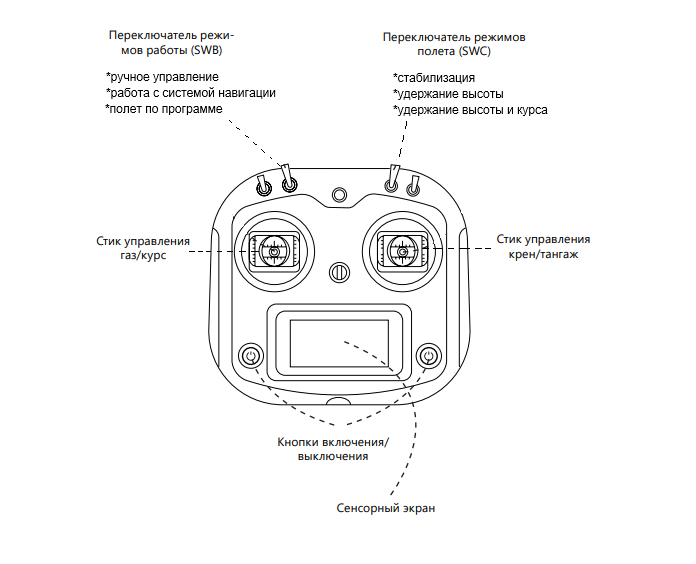
\includegraphics[width=0.8\textwidth]{images/rc_sticks_overview.png}
    \caption{Обзор органов управления пульта FS-i6S}
\end{figure}

\subsubsection{Режимы управления (Тумблеры)}

Тумблеры используются для переключения полетных режимов и активации функций. Ранее мы настроили тумблер \textbf{SwC} (трехпозиционный справа) на 5-й канал.

\textbf{Изменение режима полета (переключатель SwC):}

\begin{itemize}
    \item \textbf{Верхнее положение (Stabilize):} Режим стабилизации. Стик газа напрямую управляет мощностью моторов. Это наиболее «ручной» режим, требующий от пилота постоянного контроля высоты. Подходит для опытных пилотов.
    \item \textbf{Среднее положение (AltHold):} Режим удержания высоты. Квадрокоптер использует барометр для автоматического поддержания заданной высоты. Стик газа в центре — высота не меняется. Стик вверх — набор высоты, вниз — снижение. Это рекомендуемый режим для обучения.
    \item \textbf{Нижнее положение (Headless):} Режим удержания высоты и курса. В дополнение к удержанию высоты, упрощается навигация. Квадрокоптер «запоминает» направление, в котором он был ориентирован при включении моторов (обычно «от пилота»). В полете, независимо от того, куда повернут нос дрона, нажатие стика «вправо» заставит его лететь вправо относительно пилота.
\end{itemize}

\begin{warnbox}
    \textbf{Физика полета:} Для определения высоты полетный контроллер использует барометр, измеряющий атмосферное давление. Помните, что резкие изменения давления (например, открытие окна в помещении или сквозняк) могут быть восприняты дроном как изменение высоты, что приведет к коррекции оборотов моторов.
\end{warnbox}

\textbf{Режимы работы пульта:}
\begin{itemize}
    \item \textbf{Ручное управление:} Вы полностью контролируете дрон с помощью стиков. Режим полета выбирается переключателем SwC.
    \item \textbf{Навигация и GPS:} В режимах с использованием системы навигации или GPS квадрокоптер управляется с пульта, но автоматически удерживает высоту и позицию, если отпустить стики.
    \item \textbf{Полет по программе:} Пионер выполняет загруженную миссию. Вы всегда можете переключить тумблер режимов (например, пощелкать SwC), чтобы перехватить управление и перевести дрон в ручной режим.
\end{itemize}

\subsection{Управление}

Пилотирование квадрокоптера требует координации и понимания того, как каждое движение стика влияет на движение аппарата в пространстве. Рассмотрим управление в режиме \textbf{Mode 2}.

\subsubsection{Управление высотой (Газ / Throttle)}

Левый стик, движение вверх-вниз.

\begin{itemize}
    \item \textbf{Стик вверх:} Обороты моторов увеличиваются, подъемная сила растет, квадрокоптер набирает высоту.
    \item \textbf{Стик вниз:} Обороты уменьшаются, квадрокоптер снижается.
\end{itemize}

\begin{figure}[H]
    \centering
    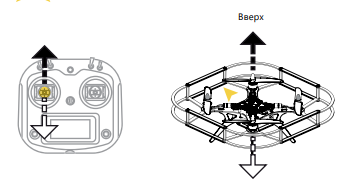
\includegraphics[width=0.45\textwidth]{images/rc_control_1.png}
    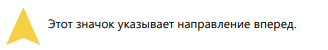
\includegraphics[width=0.45\textwidth]{images/rc_control_2.png}
    \caption{Управление газом: набор высоты и снижение}
\end{figure}

\begin{warnbox}
    \textbf{Важно:} В режиме AltHold (удержание высоты) центр стика соответствует зависанию. Для взлета необходимо поднять стик выше середины.
\end{warnbox}

\subsubsection{Вращение по курсу (Рыскание / Yaw)}

Левый стик, движение влево-вправо.

Отвечает за поворот квадрокоптера вокруг своей вертикальной оси. Это позволяет изменить направление «взгляда» дрона.

\begin{itemize}
    \item \textbf{Стик влево:} Нос квадрокоптера поворачивается влево (против часовой стрелки).
    \item \textbf{Стик вправо:} Нос квадрокоптера поворачивается вправо (по часовой стрелке).
\end{itemize}

\begin{figure}[H]
    \centering
    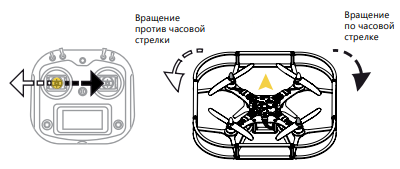
\includegraphics[width=0.75\textwidth]{images/rc_control_3.png}
    \caption{Рыскание: вращение вокруг оси}
\end{figure}

\subsubsection{Тангаж (Pitch) — Движение вперед/назад}

Правый стик, движение вверх-вниз.

Изменяет угол наклона квадрокоптера в продольной плоскости, заставляя его двигаться горизонтально.

\begin{itemize}
    \item \textbf{Стик вверх (от себя):} Нос опускается, дрон летит вперед.
    \item \textbf{Стик вниз (на себя):} Нос поднимается, дрон летит назад.
\end{itemize}

\begin{figure}[H]
    \centering
    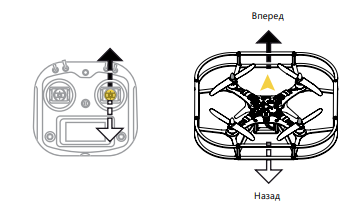
\includegraphics[width=0.75\textwidth]{images/rc_control_4.png}
    \caption{Тангаж: движение вперед и назад}
\end{figure}

\subsubsection{Крен (Roll) — Движение влево/вправо}

Правый стик, движение влево-вправо.

Изменяет угол наклона квадрокоптера в поперечной плоскости, заставляя его смещаться вбок.

\begin{itemize}
    \item \textbf{Стик влево:} Дрон наклоняется влево и летит боком влево.
    \item \textbf{Стик вправо:} Дрон наклоняется вправо и летит боком вправо.
\end{itemize}

\begin{figure}[H]
    \centering
    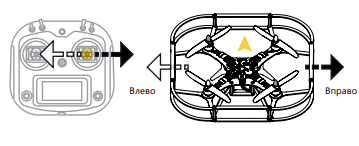
\includegraphics[width=0.75\textwidth]{images/rc_control_5.png}
    \caption{Крен: движение боком}
\end{figure}

\begin{hintbox}
    \textbf{Совет:} При обучении полетам держите хвост квадрокоптера (где установлен аккумулятор или светодиод) к себе. Так направления управления будут совпадать: стик вправо — дрон вправо. Если дрон развернется к вам носом, управление станет «зеркальным» (стик вправо — дрон влево с вашей точки зрения).
\end{hintbox}
